\documentclass[preprint,12pt]{elsarticle}

\begin{document}

\begin{frontmatter}

\title{ArtifactGate-EDA: An Adapter-Based Claim-Safe Artifact Evaluation Framework for Software-Only EDA Experiments}

\author[inst1]{Xinzhi Lei}
\affiliation[inst1]{organization={Independent research software project}}

\begin{abstract}
ArtifactGate-EDA is an open-source Python framework for claim-safe artifact
evaluation in software-only EDA experiments. It ingests heterogeneous outputs
from SPICE/ngspice, HDL simulation, and Yosys synthesis workflows; records
provenance and hashes; generates replay manifests; classifies evidence levels;
and reports unsupported claims. The software is demonstrated on bounded
software-level examples, including corrupted-artifact tests and negative
claim-injection tests. ArtifactGate-EDA does not validate hardware, Vivado
timing, DFX deployment, bitstreams, or board-level behavior.
\end{abstract}

\begin{keyword}
EDA \sep artifact evaluation \sep reproducibility \sep claim checking \sep ngspice \sep Yosys
\end{keyword}

\end{frontmatter}

\section*{Highlights}
\begin{itemize}
\item Claim-safe artifact packaging for software-only EDA experiments.
\item Adapter-based ingestion for ngspice, HDL simulation, and Yosys evidence.
\item Negative claim tests block unsupported stronger evidence claims.
\end{itemize}

\section*{Metadata}
\begin{tabular}{lll}
Nr & Code metadata description & Metadata \\
C1 & Current code version & 0.1.0 \\
C2 & Permanent repository link & https://github.com/KKKKJ687/ArtifactGate-EDA \\
C3 & Legal code license & Apache-2.0 \\
C4 & Versioning system & git \\
C5 & Languages/tools & Python, Makefile, GitHub Actions \\
C6 & Requirements & Python >=3.10; see pyproject.toml \\
C7 & Documentation & README.md and docs/ \\
C8 & Support email & Pending author-side release metadata \\
\end{tabular}

\section{Motivation and significance}
EDA artifact packages often mix source files, simulator logs, synthesis
reports, metadata, replay commands, and paper claims. ArtifactGate-EDA provides
a software layer for indexing these artifacts, assigning evidence levels,
checking claim support, and generating reviewer-readable reports.

\section{Software description}
The package provides command-line tools for ingestion, validation, replay,
claim checking, reporting, packaging, and drift comparison. Its adapter layer
covers ngspice, Icarus/VVP, Yosys, Verilator, and metadata-only supplementary
adapters.

\begin{figure}
\centering
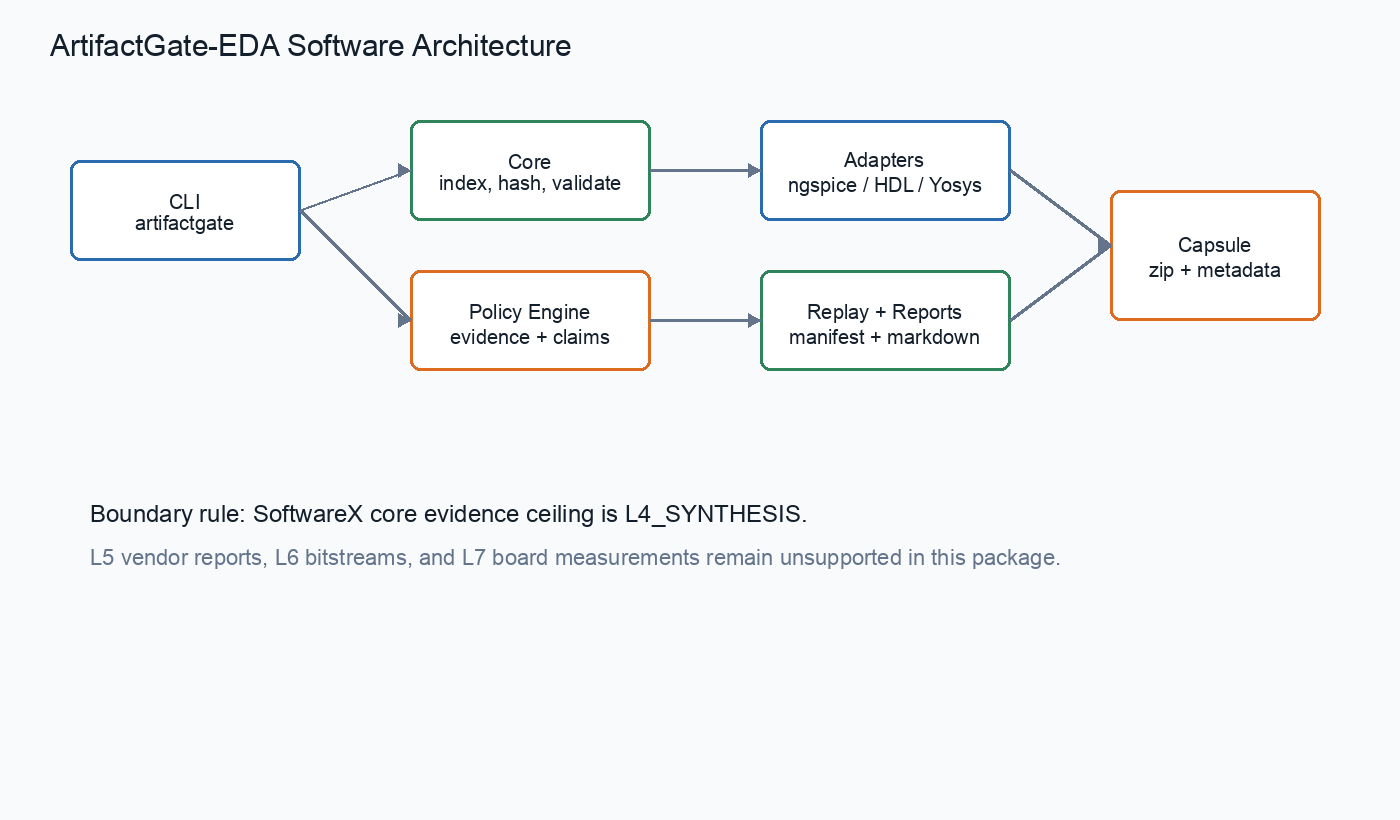
\includegraphics[width=\linewidth]{figures/architecture.png}
\caption{ArtifactGate-EDA software architecture.}
\end{figure}

\begin{figure}
\centering
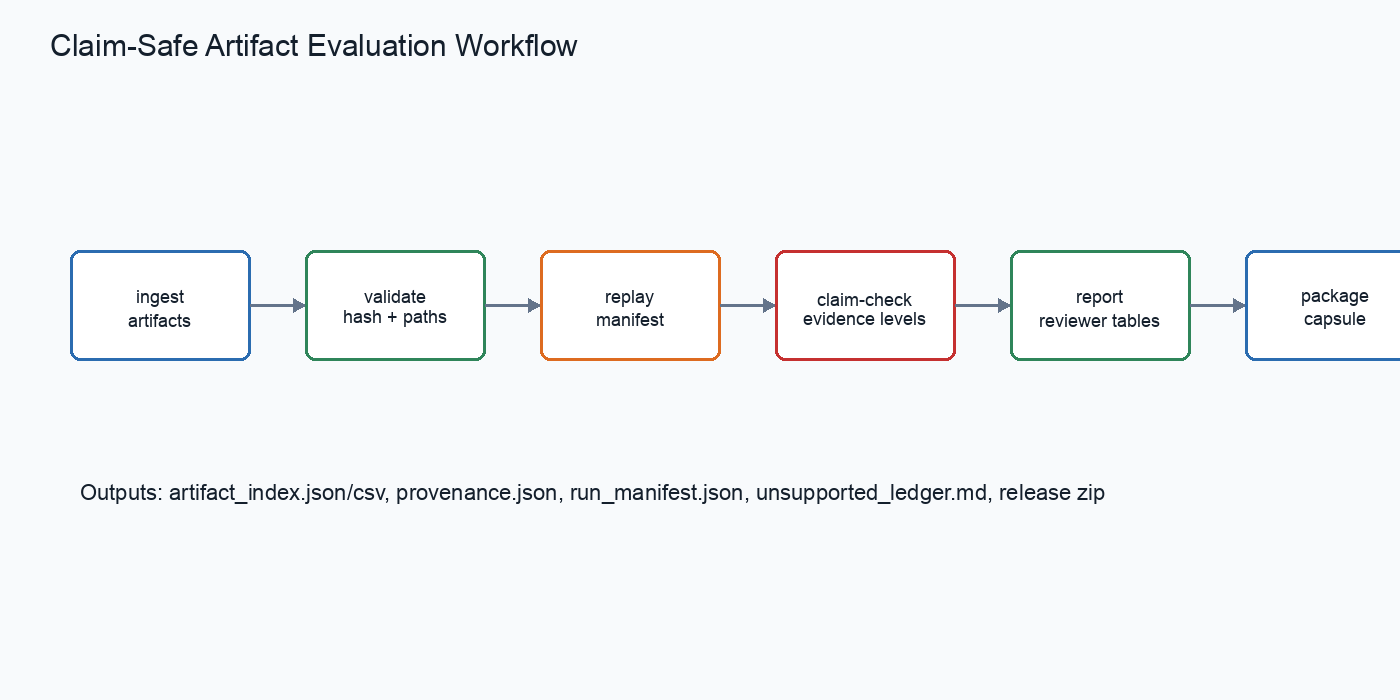
\includegraphics[width=\linewidth]{figures/workflow.png}
\caption{Claim-safe artifact evaluation workflow.}
\end{figure}

\section{Illustrative examples}
The repository includes bounded examples for ngspice-style SPICE artifacts,
HDL/Icarus simulation artifacts, Yosys synthesis artifacts, Verilator logs,
PLECS metadata-only artifacts, and Logisim metadata-only artifacts. Corrupted
artifact and negative claim examples exercise reviewer-facing failure modes.

\begin{figure}
\centering
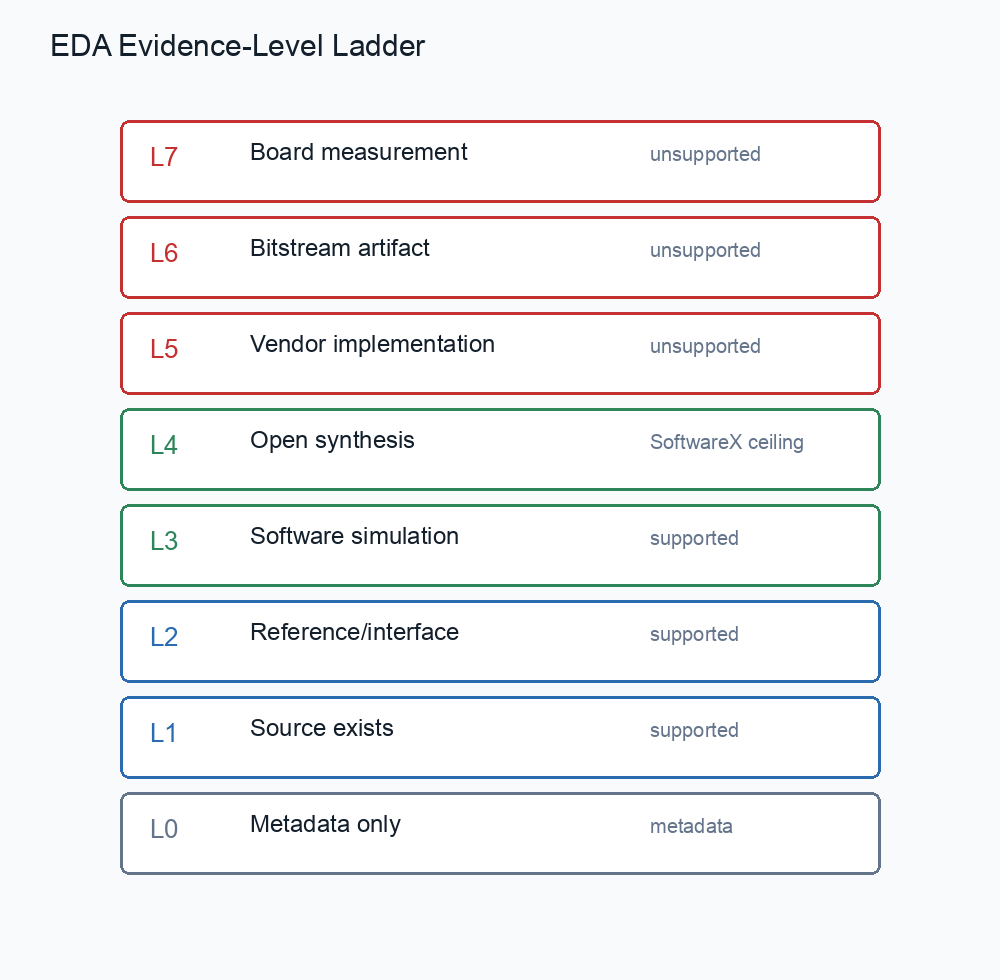
\includegraphics[width=\linewidth]{figures/evidence_levels.png}
\caption{Evidence-level ladder and the SoftwareX evidence ceiling.}
\end{figure}

\section{Impact}
ArtifactGate-EDA complements generic reproducibility tooling by adding
EDA-specific evidence levels, unsupported-claim ledgers, and reviewer-facing
artifact reports.

\section{Experimental evaluation}
The repository includes smoke tests, multi-adapter ingestion, replay checks,
negative claim injection, corrupted package detection, scalability summaries,
and artifact-management baseline comparison.

\begin{figure}
\centering
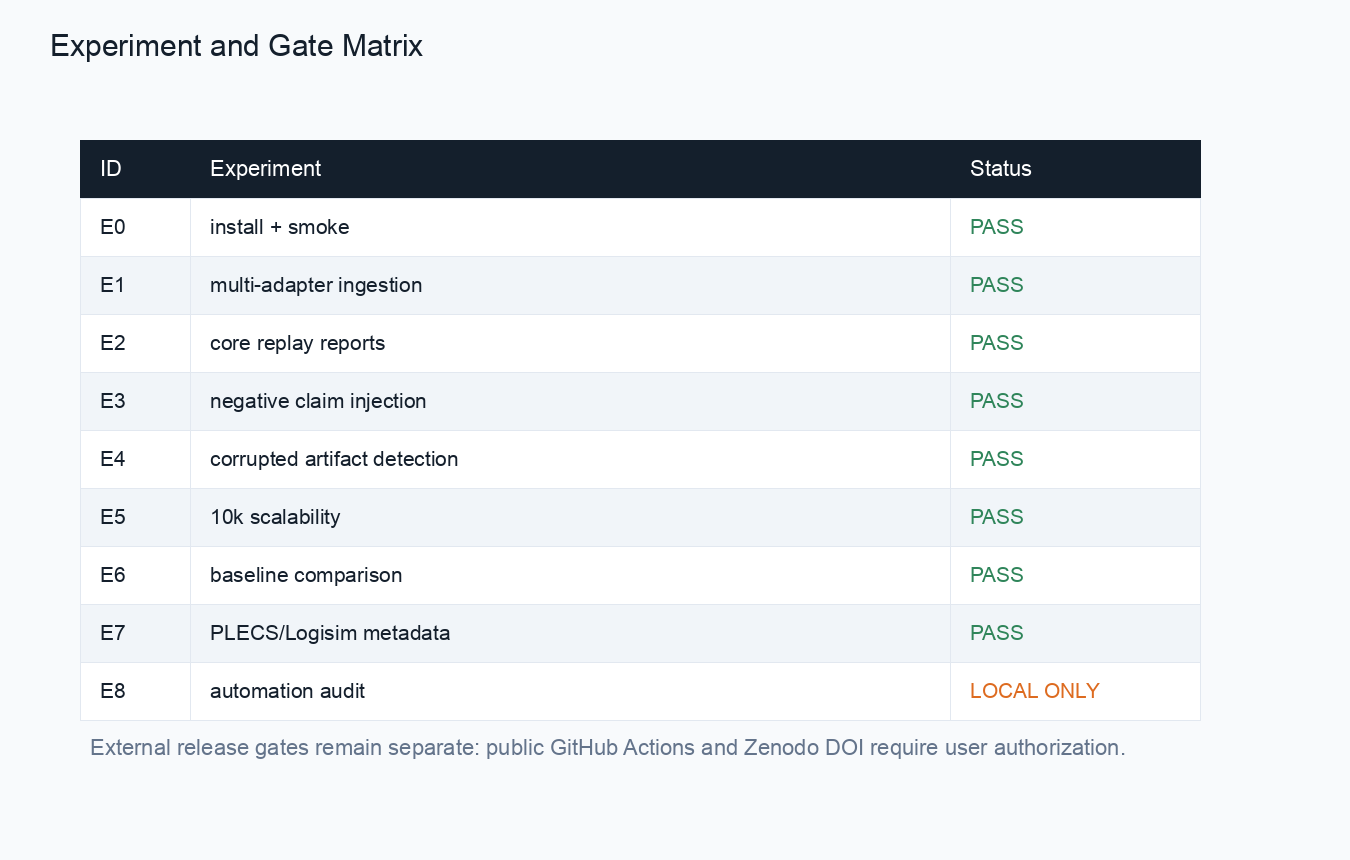
\includegraphics[width=\linewidth]{figures/experiment_matrix.png}
\caption{Local experiment and gate matrix.}
\end{figure}

\section{Conclusions}
ArtifactGate-EDA packages heterogeneous software-only EDA artifacts into
hash-recorded, replay-checkable, and claim-auditable bundles. Local evaluation
covers installation, multi-adapter ingestion, replay summaries, negative claim
injection, corrupted artifact detection, scalability summaries, and
artifact-management baseline comparison.

\section{Limitations}
The SoftwareX core is limited to software, simulation, and open-source
synthesis evidence. Stronger hardware-level claims remain out of scope unless
future releases add direct evidence and separate validation.

\section{Availability}
Repository: https://github.com/KKKKJ687/ArtifactGate-EDA. The archived Zenodo DOI
will be added before SoftwareX submission.

\end{document}
